\section{FuzzBench}
\label{sec:ch4-fuzzbench}

% -T: Explain fuzzbench

\subsection{Fuzzer Benchmarking As a Service}

\say{FuzzBench is a free service that evaluates fuzzers on a wide variety of real-world benchmarks, at Google scale. The goal of FuzzBench is to make it painless to rigorously evaluate fuzzing research and make fuzzing research easier for the community to adopt.} \cite{metzman2020fuzzbench}

\begin{figure}[!t]
    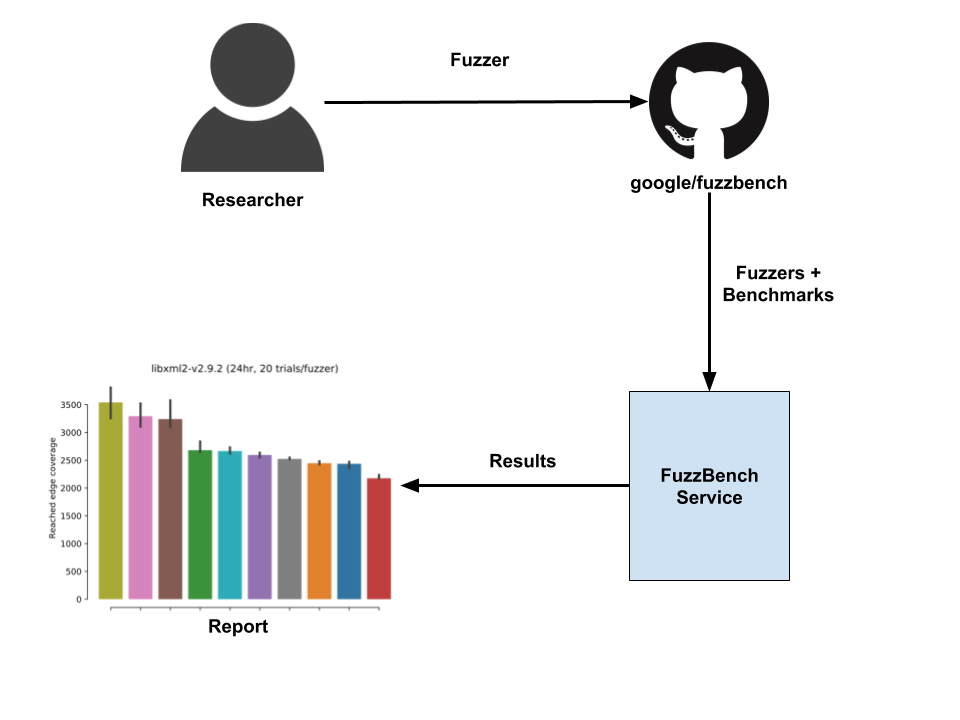
\includegraphics[width=\textwidth]{Chapter4/FuzzBench-service.png}
    \centering
    \caption{Fuzzbench overview}
    \label{fig:fuzzbench}
\end{figure}

Fuzzbench provides different modules for customized fuzzers. As illustrated in \ref{fig:fuzzbench}, we first introduce Waffle to fuzzbench by adding a directory of \texttt{Dockerfile}s, with the recipes for building and running the fuzz testing. Next, by passing the name of the fuzzers and the benchmarks, the evaluations begin to run as prescribed (3 trials, 12 hours). On the termination of all experiments, fuzzbench aggregates the performance of the fuzzers and benchmarks, and generates a comparative report of the whole benchmarking, and ranks the fuzzers based on their performance. Hence, the execution times are processed seperately for the execution time feature. In order to understand the whole procedure of testing, we explain how we have added Waffle to the system, and continue with the steps taken to get the results.

% -T: Explain the setup

\subsubsection{Add Waffle to FuzzBench}

\begin{sloppypar}
The current version of FuzzBench contains more than 30 different fuzzers available for testing. To evaluate Waffle, we need to first add Waffle to the list of known fuzzers which Fuzzbench communicates with. One of the options for adding a new fuzzer is by building a docker image, which builds Waffle project and passes \texttt{waffle-clang} compiler to fuzzbench for generating the binaries of the benchmarks. To build such docker images, we include the following files into \texttt{<fuzzbench-root>/fuzzers/waffle}:
\end{sloppypar}

\begin{itemize}
    \begin{sloppypar}
    \item \texttt{builder.Dockerfile:} This file builds the fuzzer in a docker container. Fuzzbench clones Waffle's project into the container, builds the project, and specifies a driver to provide the logs of the executions for fuzzbench. The recipe can be found in Appendix \ref{app:builder.docker}.
    \end{sloppypar}
    \item \texttt{runner.Dockerfile:} This file introduces compilation procedure for generating an instrumented binary of the target program. As Waffle is extending AFL, fuzzbench follows the same recipe, and generates the target file with the introduced (Waffle's) compiler.
    
    \item \texttt{fuzzer.py:} When fuzzbench finishes its setup for running a test, the content of \texttt{fuzzer.py} executes fuzz testing without showing the status screen, and creates running instances of the trials. [Appendix \ref{app:fuzzer.py}].
\end{itemize}

\subsubsection{Start an experiment}

We use a \textbf{local experiment} for evaluations. The local computer runs on Ubuntu 18.04 64bits, with Intel® Core™ i7-3770 CPU @ 3.40GHz × 8, and 16 GBs of RAM. The measurements for the performance of HDD, show 30MB/s for reading from the disk, and can write for 25MB/s.
